\chapter{Measurements}
\label{chap:measurements}

This chapter represents the main part of the practical work. Based on the identified metrics several measurement methods and tools are explained and the results shown and analyzed. Starting with the measurements of the time passed between the user entered the URL into her browser's address line and hit the "Enter" button and the receiving of the critical first byte on the client side we are also looking deeper into the browser processing.

\section{Leverage of fundamental Internet Protocols}
As the discussed metrics can have a huge impact on the overall web performance, we take a short look on the fundamental internet protocols involved when requesting a web page. 

\textbf{HTTP} is the main protocol responsible for delivery of a request to the server and a response back again. The method and relevant information is packed within a so called HTTP header and body. Request methods supported by every browser are GET and POST whereby GET allows to send custom parameters (data concerning the purpose of the application) within the header and POST within it's body. Furthermore the browser can add different properties to tell which version it supports, whether compression and caching can be used or TCP connections should be kept open. Adapting these properties in a web server's configuration can help to optimize performance remarkably \cite{Chang_2008}.

\textbf{TCP} is the basis for nearly all of the HTTP traffic delivered on the Internet. Changes by web engineers in HTTP configuration can influence the performance of TCP and the underlying network. TCP is very sensitive to latency as connections start with a three-way handshake between client and server to agree on connection specific variables. Since TCP is a reliable protocol it contains special algorithms to control and avoid congestions as well as handle bandwidth differences and network condition varieties appropriately. In general TCP is conservative about packet sizes to avoid overwhelming the other side and the underlying network. As a consequence transferring a bigger HTML file can easily lead to several roundtrips between the two stations \cite{Grigorik_2013}. 

\textbf{SSL} represents the security layer for HTTP requests. For several years now more and more HTTP connections are encrypted with SSL to provide encryption, authenticity and integrity. The same is the case for Tractive's web application. Despite these advantages SSL contributes to network latency a quite big part since establishing of a SSL Tunnel requires a so called SSL handshake which diminishes network latency. First Client and Server have to advertise their CipherSuites and other encryption details. In a second step they use public key cryptography to negotiate a shared secret key without any prior knowledge of each other. Then the client (and sometimes also the server) checks the identity of the other side based on verified certificates and integrity of the messages are checked via a checksum too. In total this handshake requires two full roundtrips and therefore another bunch of hundreds of milliseconds. Unoptimized SSL settings for HTTP connection can lead to performance problems when a lot connections have to be established.

\section{Comparing HTTP and HTTPS requests}
The goal of the first measurements is to split a basic HTTP request into it's single parts and to get out how much time each of them costs. 
CURL is nice and simple REST command line tool which comes with some useful options to analyze the performance of a specific request. A bash script including a custom output template provides some insights into the concerning time periods. 

\begin{table}[h]
\begin{center}
\begin{tabular}{| c | c |}
    \hline
    Time period & Time  \\ \hline
    DNS Lookup & 5ms  \\ \hline
    TCP Connect & 36ms \\ \hline
    Application Connect & 0ms \\ \hline 
    Pre Transfer Time & \textbf{36ms} \\ \hline
    Redirect & 0ms\\ \hline
    Time to first Byte & 60ms \\ \hline
    Total Time & 60ms \\
    \hline
\end{tabular}
\caption{Requesting tractive.com/en over HTTP}
\end{center}
\end{table}

\begin{table}[h]
\begin{center}
\begin{tabular}{| c | c |}
    \hline
    Time period & Time  \\ \hline
    DNS Lookup & 4ms  \\ \hline
    TCP Connect & 28ms \\ \hline
    Application Connect & \textbf{179ms} \\ \hline 
    Pre Transfer Time & \textbf{179ms} \\ \hline
    Redirect & 0ms\\ \hline
    Time to first Byte & 264ms \\ \hline
    Total Time & 321ms \\
    \hline
\end{tabular}
\caption{Requesting tractive.com/en over HTTPS}
\end{center}
\end{table}

As we can see from the results the time spent on the network is just a few milliseconds here because the network latency is not that much due to the pretty short distance between our office in Pasching and the Servers in Germany. Despite it takes 29ms in the first test to establish the underlying TCP connection. The main page which was requested here does not require much work on the server since only the HTML page using the correct language file for the text (English in this case) has to be generated by the Rails application server. This happens in moderate time in both cases. Fortunately the bandwidth in the office network is quite high and the Wi-Fi connection stable so the content is downloaded really fast. What makes a big difference is the use of an SSL Tunnel for the HTTP request. Although the propagation latency is just a few milliseconds due to the short distance the two extra roundtrips as mentioned earlier lead to a noticeable drawback. Luckily the evolvement of SSL improved the handshake procedure a lot so that it's not necessary for instance to do the same algorithm for every established TCP connection.

\section{Measuring with Apache Benchmark}

CURL is a convenient tool to get some quick information about REST calls and enables us to look at some performance indicators. However, for further performance tests it is not well suited and therefore the Apache Benchmark (shortly called AB) is my choice. It's a command line tool as well which gives a rich set of information out-of-the-box and can be effectively used in custom performance scripts. Since scalability for well-visited web applications is essential for any successful web business the following tests try to figure out how the involved components and the network time gets affected under increasing load by comprehensive measurements. This method is also called load testing.

Example for a simple ab test triggering 100 requests whereby there are 10 concurrent ones using HTTP keep-alive to perform multiple requests within one HTTP session.
\begin{lstlisting}
ab -kn 100 -c 10 https://tractive.com/en/
\end{lstlisting}

The following parts look at some of the measurement results in more detail.
Therefore I will show and analyze primarily the time periods named connection, processing, waiting and total time to first byte.

\textbf{Connect:} Network latency plus overhead to establish connection to remote host which includes establishing DNS lookup, TCP connection and SSL handshake.
\textbf{Processing:} This is the server response time. The time it took the server to process the request and send a reply.
\textbf{Waiting:} Time between sending the request from client to server plus time after processing until receiving of first byte.
\textbf{Total:} Sum of Connect + Processing which equals the Time to first byte.

\subsection{Sequential requests of different pages}
First of all I compare the sequential requests of the page which shows the Tractive mobile apps and the page which shows the Tractive tracker devices.

\begin{figure}[h!]
	\centering
		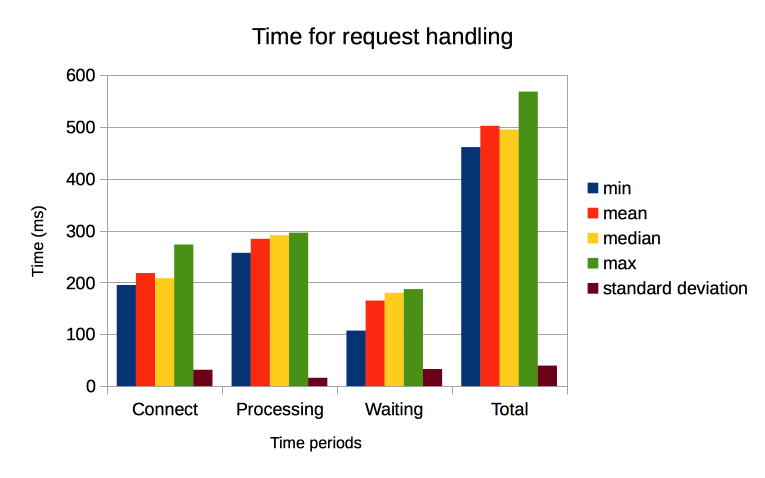
\includegraphics[width=0.9\textwidth]{imgs/seq_req_apps.png}
	\caption{Five sequential requests to https://tractive.com/en/apps}
\end{figure}

\begin{figure}[h!]
	\centering
		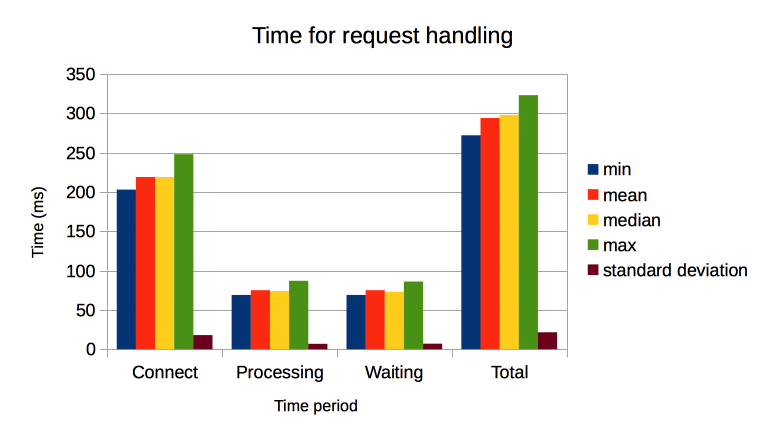
\includegraphics[width=0.9\textwidth]{imgs/seq_req_trackers.png}
	\caption{Five sequential requests to https://tractive.com/en/trackers}
\end{figure}

As we can see from the results, the processing and waiting time mainly depends on the type and content of the page. The apps page requires due to its nature more processing work on the server than the trackers page and therefore there is this difference. The connection time in contrast stays pretty consistent at a median of approximately 215ms. This does not change with content or processing time on server, it depends on latency. This fact furthermore emphasizes how important network latency is to provide a fast Time to first byte.

\subsection{Load testing with concurrent requests}
With concurrent requests you can stress the web servers as well as the underlying network including intermediate routes on the way. Although I did some measurements with a rather unrealistic number of concurrent and sequential requests for the same page it's quite interesting to see how it affects the time indicators. The pictures below illustrate performance under heavy concurrent load and shows the development in case of increasing concurrency.

\begin{figure}[h!]
	\centering
		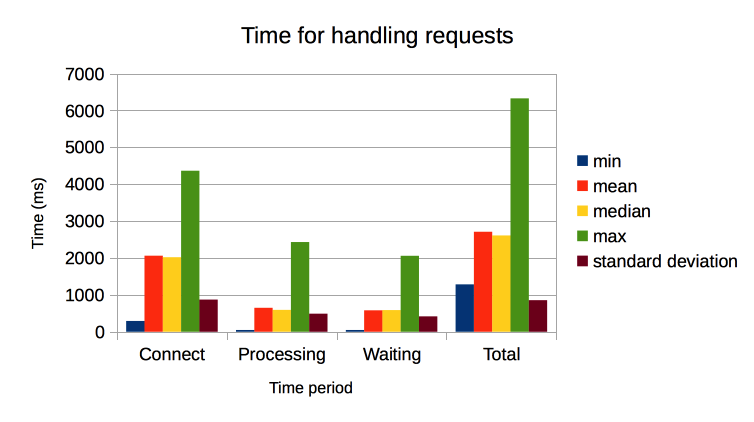
\includegraphics[width=0.9\textwidth]{imgs/con_req100.png}
	\caption{Requesting https://tractive.com/en with 1000 requests - 100 concurrently}
\end{figure}

\begin{figure}[h!]
	\centering
		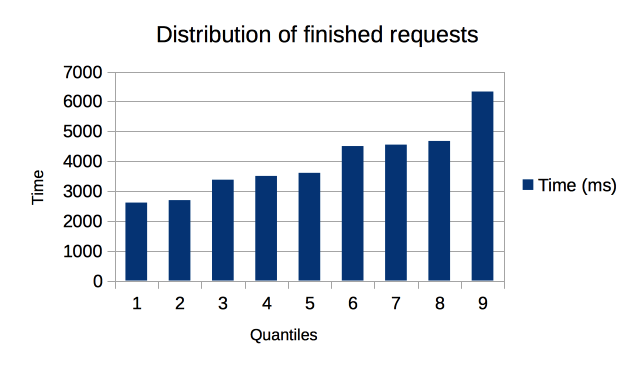
\includegraphics[width=0.9\textwidth]{imgs/dist_con100.png}
	\caption{Distribution of processed requests}
\end{figure}

\begin{figure}[h!]
	\centering
		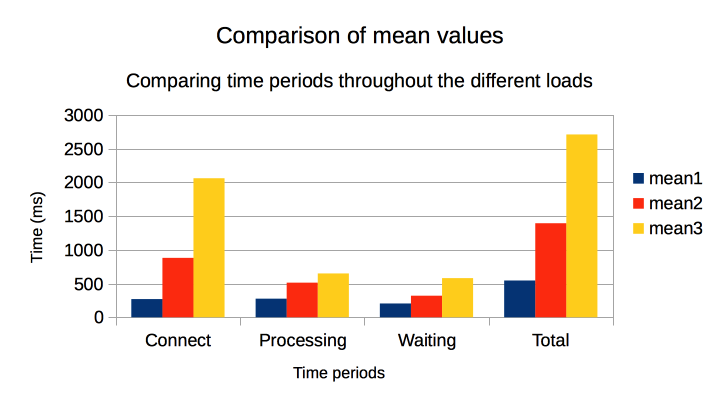
\includegraphics[width=0.9\textwidth]{imgs/comparison_mean_values.png}
	\caption{Comparing mean values for increasing concurrency resp. amount of requests}
\end{figure}

The results show that the standard deviation becomes really high especially for the connection setup time which means that the network is unpredictable. Most likely packets pile up at intermediate hops and get queued or TCP connection set-up slows down due to the enormous amount of requests in such a short time window. Whereas the standard deviation for the processing time remains lower. The redundancy of three multi-purpose application hosts with the HAProxy as load balancer takes some load off each instance. In the distribution graph you can see that it takes quite a long time to finish the last percent of requests because there are some extreme outliers. The metric $$\frac{median}{minimum}$$ gives a good indicator whether data points are clustered around the median, the server is operating normally and can handle requests with similar balance. The optimum would be a result around 1 which in this case is absolutely not the case. The last graph tops the load testing with concurrent requests off by showing the negative development by increasing load.
Tractive uses New Relic as it's main application monitoring system. All services can be monitored effectively within this system including alarms when thresholds are exceeded. It also gives some insights into performance of the website and figure \ref{fig:newrelic2} shows the impact on network time during one of my load tests.

\begin{figure}[h!]
	\centering
		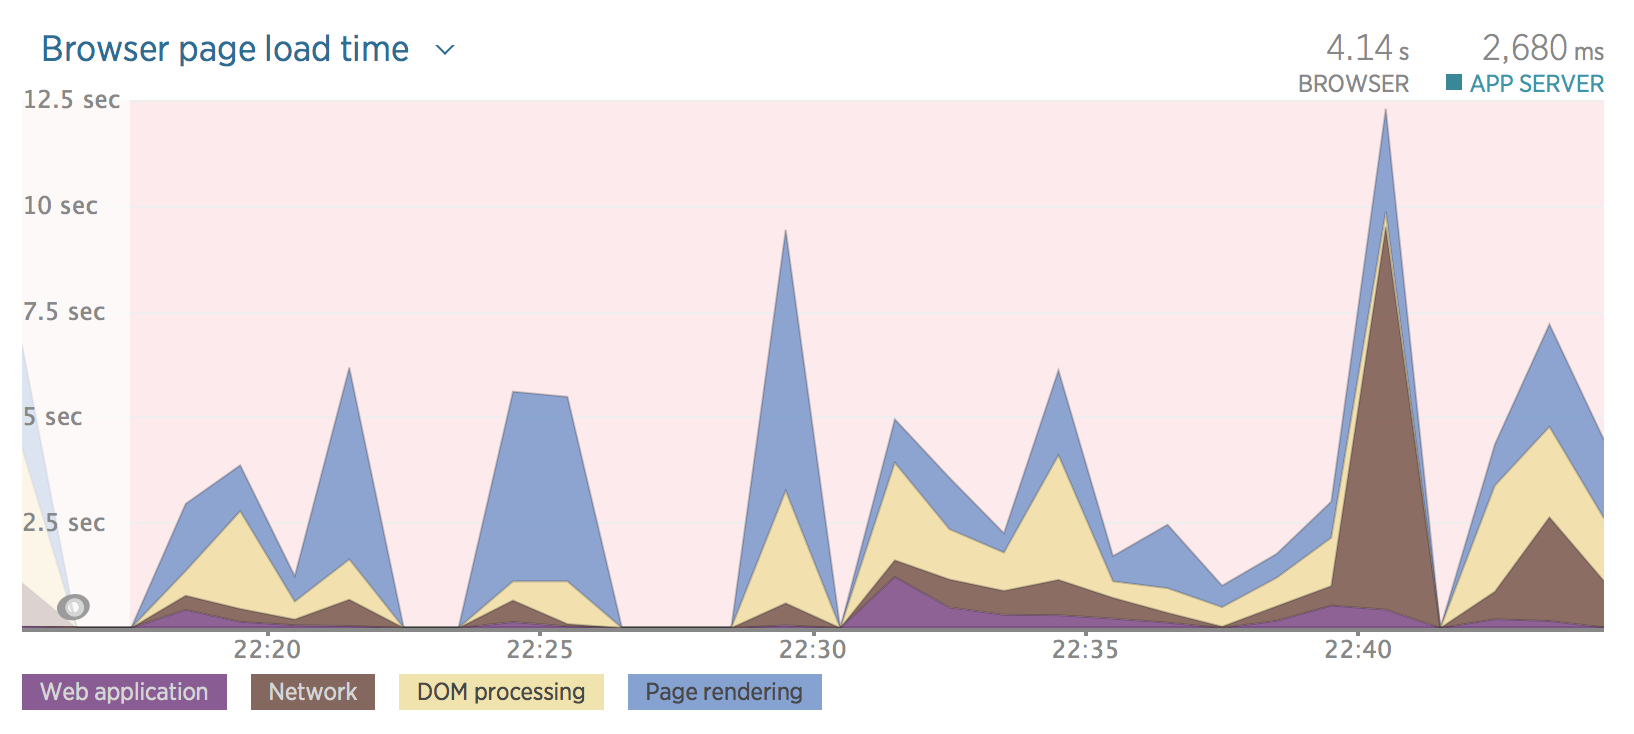
\includegraphics[width=0.9\textwidth]{imgs/newrelic_load.png}
	\caption{Web Performance Monitoring with New Relic}
	\label{fig:newrelic2}
\end{figure}  

\subsection{Consistency of performance results}
This test should analyze whether the total time (sum of connection setup and processing time) stays consistent among requests or if there is any unexpected outlier. 
A customizable bash script allows to fire a fixed amount of sequential requests in regular time periods. Following there is a short code snippet.

\begin{lstlisting}
for i in `seq 1 $1`
do
	ab -kn $2 https://tractive.com/en
	sleep $3
done 
\end{lstlisting}

To improve readability of the graph the executed performance test considers the total time of 15 requests of the same page each delayed by 5 seconds.

\begin{figure}[h!]
	\centering
		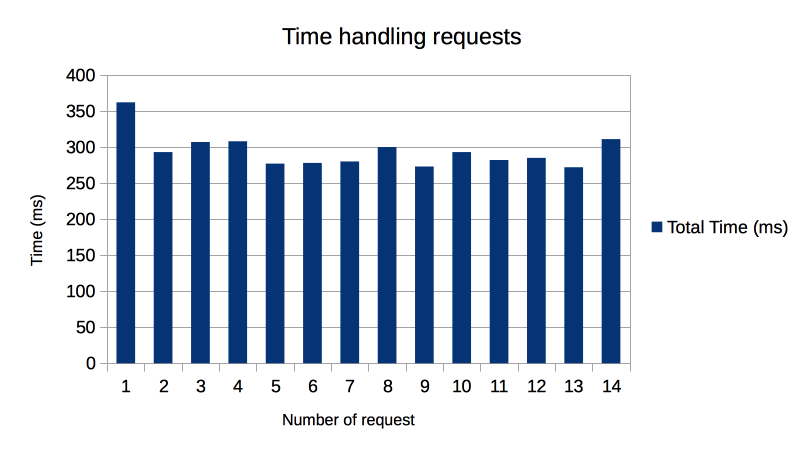
\includegraphics[width=0.9\textwidth]{imgs/consistency.png}
	\caption{Consistency throughout the requests - https://tractive.com/en}
\end{figure}

Except the first request the total times are pretty consistent around 300ms which is good. The processing and waiting times are pretty equal throughout all requests. This indicates that the server can handle the tested sequential requests without any problems over the provided time frame. Only the connection time of the very first request is approximately 50-70ms longer than the connection time of the successive requests. This behaviour is not completely clear but I suppose this is due to a DNS lookup at the first request which does not have to be done for the following requests.  

\subsection{Performance regarding daytime}
Since page load time and especially the processing of a requests also depends on the current load of the server as we have seen from previous load tests. Customer activity can also vary throughout the daytime and regarding the Tractive Web application it can be assumed that most users are online during the day since the dominant user basis is within Europe. The following measurements should find out whether this fact actually has an impact on the network and server performance. The results of the performance test are compared and displayed in the graph below.

\begin{figure}[h!]
	\centering
		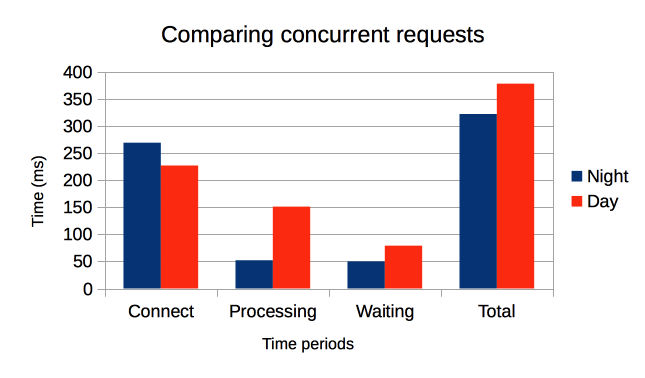
\includegraphics[width=0.9\textwidth]{imgs/day_night_con.png}
	\caption{Comparing 100 requests - 10 concurrently during day and night (10:25am, 11:15pm) - https://tractive.com/en/apps}
\end{figure}

Although the results are pretty similar the processing and waiting time is less during the night supporting the initial assumption. However, for a secure prove of this fact other metrics, such as the current number of users at the concerned time, have to be considered and several measurements under similar circumstances should be taken.

\section{Measure Browser Processing}
\label{sec:browserProcessing}

We heard a lot about network latency, time spent establishing connections and handshakes. This section shows the second big part of my measurements which is the performance of downloading resources like HTML, Javascript or Images and displaying the result in the browser. As mentioned in section \ref{sec:browserproc} there is usually a lot of work for the browser to render the page successfully and web developers can optimize some things here to improve the user experience. webpagetest.org is a rich tool to analyze the web performance. It gives deep insights in the building process and reveals possible problems or bottlenecks. Since Tractive is a globally operating company it is very interesting to see how the performance behaves when requesting it from the USA or even Australia. I considered this in my tests as well to show how it affects the loading times and emphasizes possible problems. Figure \ref{fig:sydney_old} shows the results when requesting the main webpage from Sydney, Australia.

\begin{figure}[h!]
	\centering
		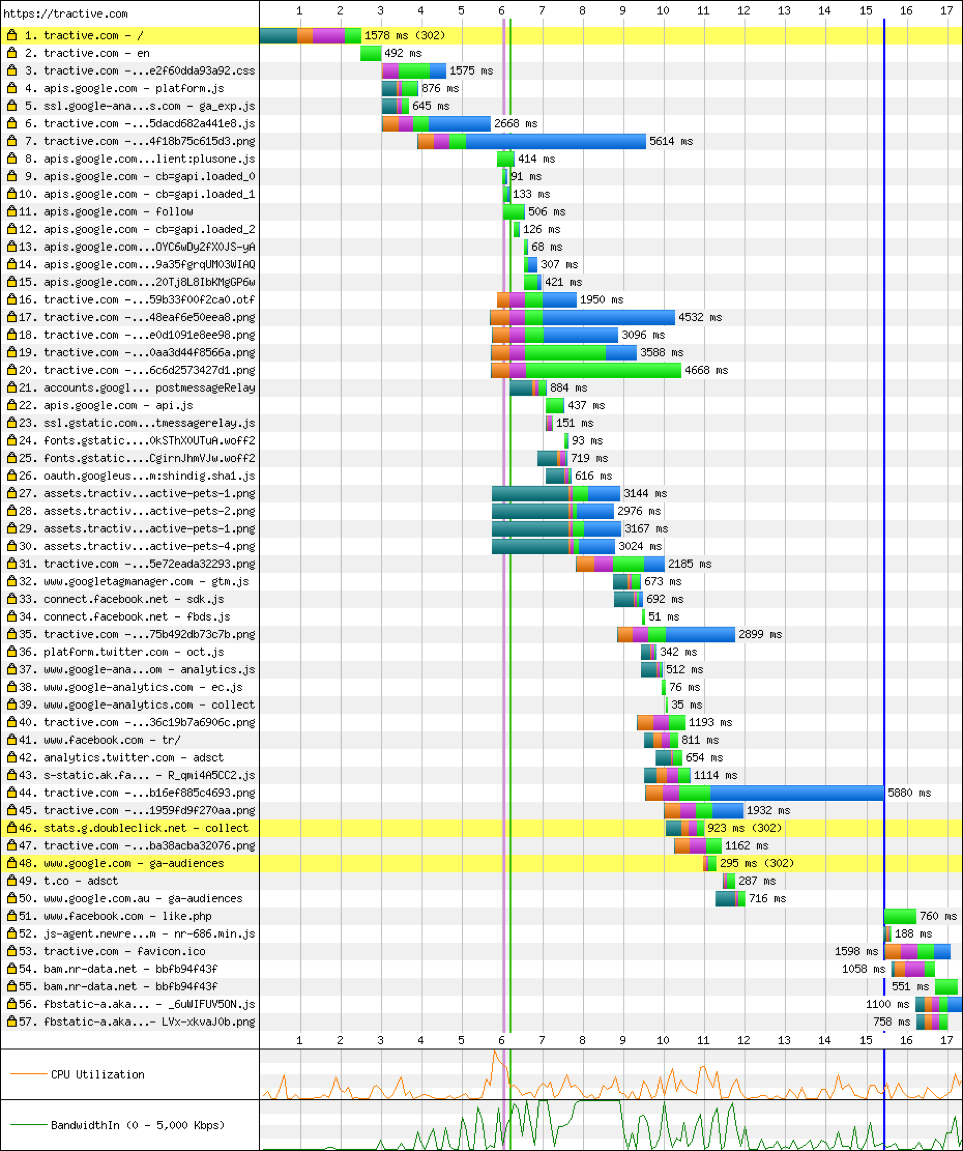
\includegraphics[width=0.9\textwidth]{imgs/webpagetest_old_sydney.png}
	\caption{Waterfall view of https://tractive.com - Request from Sydney, Australia}
	\label{fig:sydney_old}
\end{figure}

First of all the results provide an overview on important metrics starting with \textbf{Load Time} which indicates the duration until the page is completely rendered and no further work has to be done. The \textbf{First Byte} is the well discussed time when the first byte has arrived on the client. Until this point of time the browser can't do anything and just \textbf{Start Render} indicates when the browser starts rendering the first element on the screen. It is crucial because until this point of time the user starres at a blank page and just sees the circling spinner. We can see from the second table that prior to Start Render the domContentLoaded event is fired and therefore empasizes how important it is to get the DOM ready as soon as possible. The \textbf{Visually complete} time is just an indicator from webpagetest.org when the filmstrips taken are complete. More important are the columns \textbf{Document Complete} showing the number of requests, content downloaded and once again onLoad time respectively Fully Loaded including further requests after the document is loaded and rendered completely, as the favicon for instance. 

The waterfall view shows each request with it's according time periods explained in the legend above. Already the first request introduces a time delay of 1578ms although it just retrieves a frew bytes. This heavily reflects our knowledge and results from the previous measurements because it is mainly latency which makes the difference here. Before any resources are downloaded a second request does a redirect to the desired language based on the Accept-Language: en-US,en;q=0.8 header from the first request. This is a problematic request since it basically does nothing and costs nearly half a second. Finally the first byte has received at the browser and it now can start downloading necessary resources and building DOM and CSSOM. CSS and Javascript are critical resources because they block DOM creation and therefore delay the Start Render time. For formatting the page we have to load the application.css at the beginning followed by some Javascript files needed for Google Analytics and Google+ integration. They can be downloaded in parallel and does not introduce a big problem in this case because the application.css needs more time. A better option here is to defer loading of these Javascript files to a later time as we will discuss in \ref{chap:improvements} .However, the most critical asset here is the application.js file which contains a lot of custom Javascript functions including third party libraries like jQuery implementing client side logic and interactivity as well as AJAX and REST calls. It needs 2668ms to be downloaded and during this time the Javascript Engine is blocking DOM construction. During my further measurements I identified this asset as a potential bottleneck. Optimizing it can lower the Start Render time significantly and therefore makes the first elements of the page faster visible. Subsequently the rest of the DOM can be constructed and the green vertical line shows when the rendering of the page begins. Now all images can be downloaded and placed correctly. As expected the header takes very long to be downloaded since it is one of the biggest assets. Luckily it starts downloading pretty early to be finished in time because it represents the company and is an essential part of the main webpage. A little surprising is that the wooden background of the website is delayed until the 35th request what is probably not an optimal order. A closer look at the graphs at the bottom of the figure shows the CPU utilization during page load. There can be different reasons for high CPU utilization but usually Javascript consumes CPU a lot due to executions of functions which do computations, loop operations with higher complexity etc. In this test it shows a similar behaviour as the loading and execution of application.js introduces a peak here. Concluding this test I identify the initial redirect and the Javascript execution as major bottlenecks and therefore I will look at this in more detail in chapter \ref{chap:improvements}. 

\section{Utilization measurements}
Sometimes server capacities can introduce a bottleneck when load is too huge or other resources affect the server. This sections gives a short overview on the utilization values I found out for our three multi purpose application servers.  A very convenient command to get the most essential utilization metrics is the \textbf{top} command available in all Linux environments.

A first thing was to compare the three servers regarding their common metrics given by top:
\begin{lstlisting}
tractive03
top - 13:17:18 up 215 days,  8:02,  1 user,  load average: 2.53, 2.84, 2.77
Tasks: 222 total,   3 running, 219 sleeping,   0 stopped,   0 zombie
Cpu(s): 13.0 us,  1.7 sy,  0.0 ni, 84.7 id,  0.0 wa,  0.0 hi,  0.7 si,  0.0 sKiB Mem:  32639696 total, 25521968 used,  7117728 free,       48 buffers
KiB Swap: 16768892 total,  1242236 used, 15526656 free.  7597212 cached Mem

tractive04
top - 13:17:31 up 38 days,  2:47,  1 user,  load average: 1.60, 2.75, 2.77
Tasks: 218 total,   2 running, 216 sleeping,   0 stopped,   0 zombie
Cpu(s): 23.2 us,  3.9 sy,  0.0 ni, 72.1 id,  0.0 wa,  0.0 hi,  0.7 si,  0.0 s
KiB Mem:  49453844 total, 38325948 used, 11127896 free,       64 buffers
KiB Swap: 25149308 total,  1103168 used, 24046140 free.  9939060 cached Mem

tractive02
top - 13:17:24 up 466 days,  5:56,  1 user,  load average: 2.14, 1.79, 1.66
Tasks: 244 total,   1 running, 243 sleeping,   0 stopped,   0 zombie
Cpu(s): 27.7 us,  1.2 sy,  0.0 ni, 70.8 id,  0.0 wa,  0.0 hi,  0.3 si,  0.0 s
KiB Mem:  32808072 total, 28066204 used,  4741868 free,       68 buffers
KiB Swap:  8384444 total,  1734596 used,  6649848 free.  6363004 cached Mem
\end{lstlisting}
As expected the servers operate pretty equal and therefore no application server seems to suffer from any problem. tractive04 has with 48GB of RAM the highest capacity and uses the most memory with approximately 38GB. The average load is nearly the same on every server due to the load balancer components. The same applies for CPU utilization which emphasizes the fact that there is no strange problem on any server affecting the web performance. The load average displays three numbers whereby the first one is the average in the last minute, the second in 5 minutes and the third one spans over the last 15 minutes. The numbers indicate the average amount of processes which were waiting for the CPU. Due to the fact that these servers use 4 cores there is nearly no process which has to wait for the CPU. In addition to that it gives information about uptime, amount of tasks and following this overview a detailed list of processes and their CPU respectively memory consumption. During my investigation I did not find any processes with uncommon behaviour.  
